%!TeX root = pcb_layout
\documentclass[../main.tex]{subfiles}

\begin{document}
    \section{Thermal via for TO-263/D2PAK}
    The TO-263/D2PAK footprint is shown in Figure \ref{fig:d2pak}. Due to the existence of $R_{ds}$ of the MOSFET, there will be power loss in terms of heat. The large exposed metal back side of the TO-263/D2PAK can be taken advantage for heat dissipation. Using via, the dissipation surface of the device is extended to both side of the PCB. This method has been used extensively in industrial settings, as well as being thoroughly investigated \cite{InfineonD2PAKThermal}. In this project, each MOSFET has a 4x4 matrix of vias with $24mil$ drill size. Furthermore, the thermal dissipation area are exposed on the bottom side (See in Figure)
    \begin{figure}[!h]
        \centerline{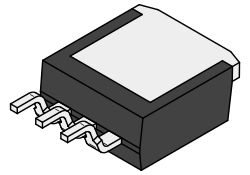
\includegraphics[width=0.5\linewidth]{media/d2pak_footprint.png}}
        \caption{TO-263/D2PAK footprint.}
        \label{fig:d2pak}
    \end{figure}

    \begin{figure}[!h]
        \centering
        \begin{minipage}{.4\textwidth}
          \centering
          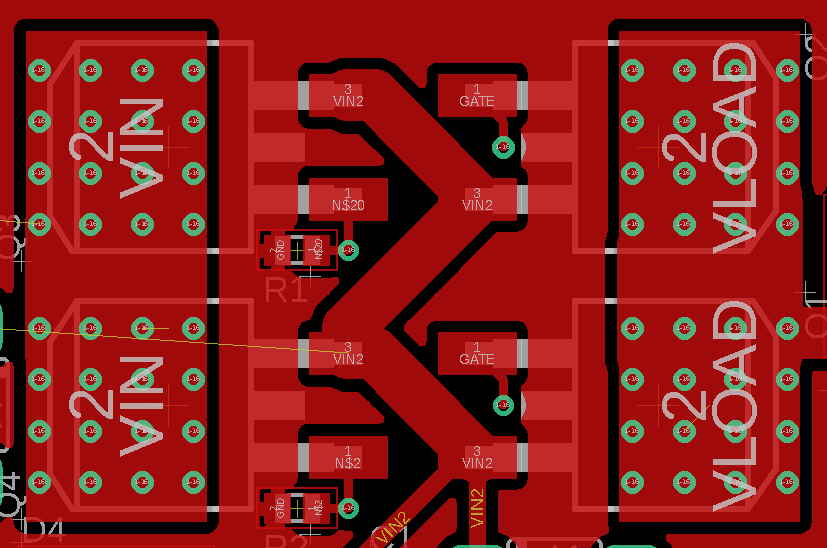
\includegraphics[width=\linewidth]{media/d2pak_thermal_vias_top.png}
        \end{minipage}\qquad
        \begin{minipage}{.4\textwidth}
          \centering
          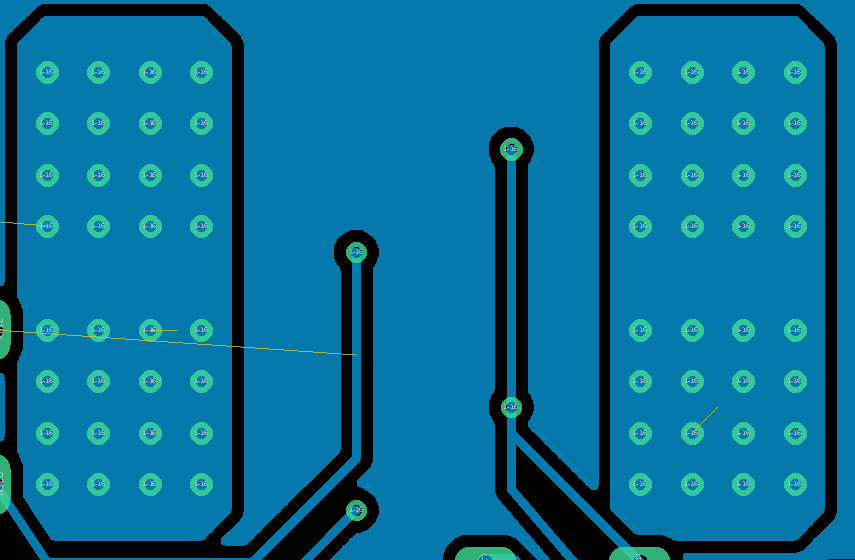
\includegraphics[width=\linewidth]{media/d2pak_thermal_vias_bottom.png}
        \end{minipage}
        \caption{Implemented PCB heat dissipation for TO-263/D2PAK footprint.}
    \end{figure}

    \pagebreak
    \section{Amass XT60PW connector}
    The following are the key features of the Amass XT60PW:
    \begin{itemize}
        \item Directional. The connector is desgined so that chances of reverse polarity connection is minimized.
        \item Anti-spark. The contactors are located so that they are covered once in contact with one another.
        \item Pressed fit connection. This allows for tight connection, while ease of removal is still guaranteed. 
    \end{itemize}
    \begin{figure}[!h]
        \centerline{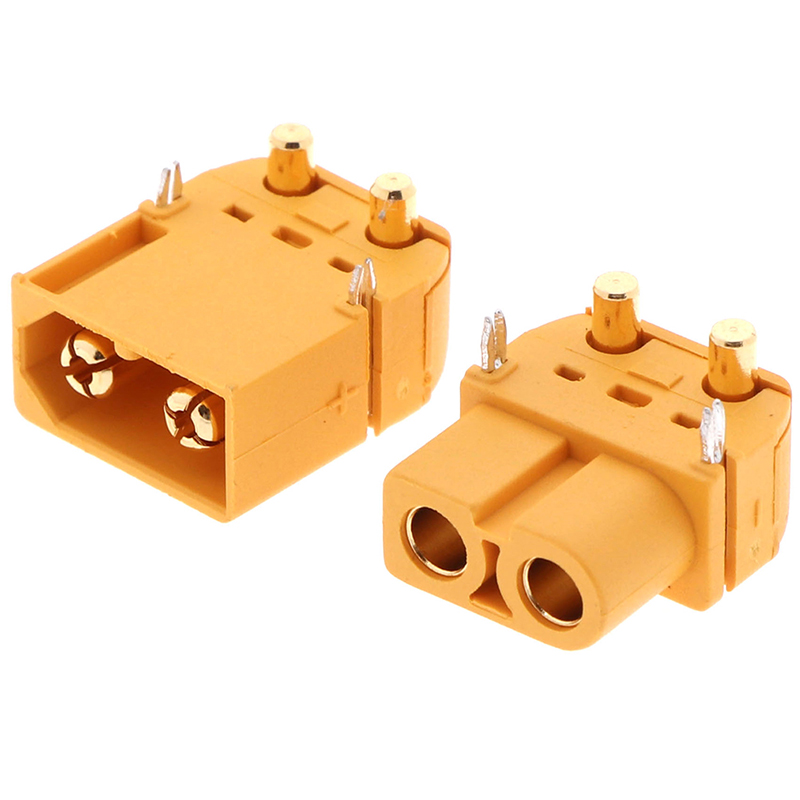
\includegraphics[width=0.5\linewidth]{media/XT60PW.png}}
        \caption{XT60PW female (left) and male (right) connector.}
        \label{fig:XT60PW}
    \end{figure}
\end{document}